% sudo apt-get install texlive-latex-base
% sudo apt-get install texlive-fonts-extra
% sudo apt-get install texlive-latex-recommended
% sudo apt-get install texlive-lang-cyrillic

%------------------------------------------------------------------------------

\documentclass[11pt]{beamer}
\usetheme{Boadilla}
\usefonttheme{professionalfonts}
\usefonttheme[onlylarge]{structurebold}
\setbeamertemplate{navigation symbols}{}

%------------------------------------------------------------------------------

\usepackage[utf8]{inputenc} % возможность использования Unicode-символов в исходных файлах

\usepackage{amsmath} % для поддержки расширенных математических символов
\usepackage{amsfonts} % для поддержки математических шрифтов
\usepackage{amssymb} % для поддержки расширенных математических символов
\usepackage{color} % для поддержки цветного текста
\usepackage{graphicx} % для поддержки рисунков

\usepackage[english,russian]{babel} % поддержка переносов слов

%------------------------------------------------------------------------------

\title[]{Минимаксная классификация интервальных оценок предпочтений с использованием машины опорных векторов}
\author[И.Ю.~Ботян, Л.В.~Уткин]{И.Ю.~Ботян\andЛ.В.~Уткин}
\institute[СПбГЛТУ]{\large Санкт-Петербургский государственный лесотехнический университет}
\date[NSMV-2014]{\large NSMV-2014, Санкт-Петербург, 27-28 июня 2014}

%------------------------------------------------------------------------------

\DeclareGraphicsExtensions{.png}

\newcommand{\Rho}{%
	\mathcal{P}%
}

%------------------------------------------------------------------------------

\begin{document}

\graphicspath{ {./img/} }

%------------------------------------------------------------------------------
\begin{frame}

\titlepage

\end{frame}
%------------------------------------------------------------------------------
\begin{frame}{Задача классификации}

\begin{itemize}
	\item Классы определяются экспертами (\textcolor{green}{зелёный} и \textcolor{violet}{фиолетовый})
	\item Использование обучающей выборки (чёрный)
	\item Задача - нахождение разделяющей функции (\textcolor{blue}{синий})
	\item Цель - соотносение объекта к тому или иному классу (\textcolor{red}{красный})
	\begin{center}
		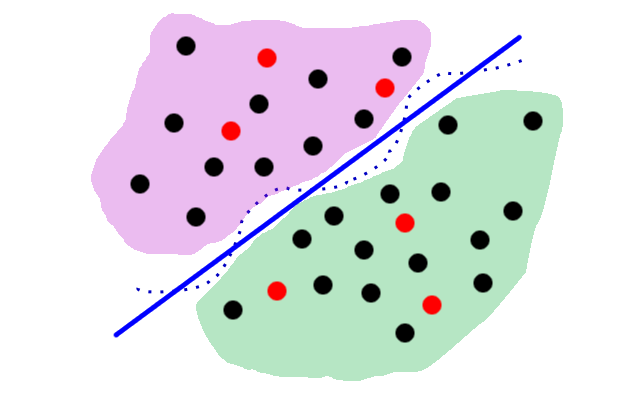
\includegraphics[scale=0.35]{classification}
	\end{center}
\end{itemize}

\end{frame}
%------------------------------------------------------------------------------
\begin{frame}{Групповые экспертные оценки}

\begin{itemize}
	\item Простая экспертная оценка - ``объект - объект''
	\item Групповая экспертная оценка - ``группа - группа''
	\begin{center}
			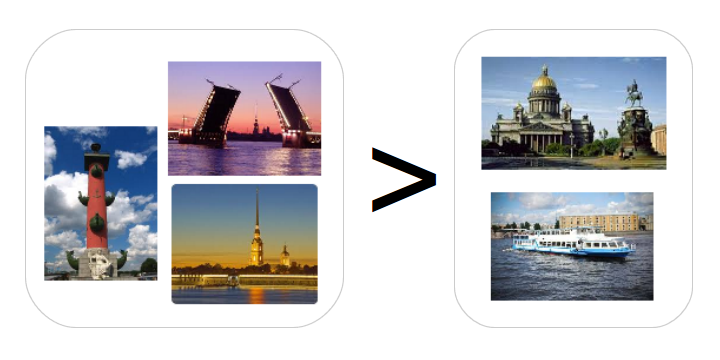
\includegraphics[scale=0.4]{interval_judgment}
		\end{center}
	\item \textbf{Пример:} планирование туристического маршрута
\end{itemize}

\end{frame}
%------------------------------------------------------------------------------
\begin{frame}{Теория Демпстера-Шефера}

\begin{itemize}
	\item Позволяет вычислять вероятность события в условиях неполной информации, комбинируя её отдельные части
	\item Неточная информация в виде неточных оценок образует множество вероятностных распределений \linebreak
	\item Верхнее и нижнее математические ожидания:
	\begin{center}
	\(\mathbb{\overline{E}} h = \sum \limits_{i=1}^N m(A_i) \inf_{x \in A_i} h(x)\) \linebreak
	\(\mathbb{\underline{E}} h = \sum \limits_{i=1}^N m(A_i) \sup_{x \in A_i} h(x)\)
	\end{center}
\end{itemize}

\end{frame}
%------------------------------------------------------------------------------
\begin{frame}{Машина опорных векторов}

\begin{itemize}
	\item Используется в качестве средства обучения
	\item Применяется метод RankSVM, основанный на попарном подходе
	\item Задача классификации - минимизация ожидаемых потерь в результате неправильной классификации пар оъектов разделяющей функцией \linebreak
	\item Минимизация функционала риска:
	\begin{center}
	\(R_{emp}(\mathbf{w}) = n^{-1} \cdot \sum \limits_{k=1}^n L(f_k, \mathbf{x}_k, y_k)\)
	\end{center}
\end{itemize}

\end{frame}
%------------------------------------------------------------------------------
\begin{frame}{Формальная постановка задачи в терминах неточных сравнений}

\begin{itemize}
	\item Есть 2 вероятностных распределения - минимизирующий и максимизирующий функционал риска
	\item Нижние и верхние границы функционала риска соответствуют верхним и нижним математическим ожиданиям в рамках теории Демпстера-Шефера:
	\begin{center}
		\(\underline{R}(\mathbf{w}) = \mathbb{\underline{E}}L = \frac{1}{n} \sum \limits_{(i,j) \in \Rho} \underset{\mathbf{x} \in \mathbf{A_i}, \mathbf{z} \in \mathbf{B_j}}{\operatorname{min}}L(f(\mathbf{x}, \mathbf{w}) - f(\mathbf{z}, \mathbf{w}))\) \linebreak
		\(\overline{R}(\mathbf{w}) = \mathbb{\overline{E}}L = \frac{1}{n} \sum \limits_{(i,j) \in \Rho} \underset{\mathbf{x} \in \mathbf{A_i}, \mathbf{z} \in \mathbf{B_j}}{\operatorname{max}}L(f(\mathbf{x}, \mathbf{w}) - f(\mathbf{z}, \mathbf{w}))\)
	\end{center} \linebreak
	\item Их выбор обуславливает стратегию принятия решений
\end{itemize}

\end{frame}
%------------------------------------------------------------------------------
\begin{frame}{Минимаксная стратегия}

\begin{itemize}
	\item \textbf{Задача} - выбор ``наихудшего'' распределения, обеспечивающего наибольшоее значение функционала риска:
	\begin{center}
	\(G_{ij} = \underset{\mathbf{x} \in \mathbf{A_i}, \mathbf{z} \in \mathbf{B_j}}{\operatorname{max}} L (f (\mathbf{x}, \mathbf{w}) - f(\mathbf{z}, \mathbf{w}))\) \linebreak
	\(\overline{R}(\mathbf{w}) = \underset{\mathbf{w}, G_{ij}}{\operatorname{min}} \sum \limits_{(i, j) \in \Rho} G_{ij}\)
	\end{center}
	\item Получена задача линейного программирования
\end{itemize}

\end{frame}
%------------------------------------------------------------------------------
\begin{frame}{Формулировка машины опорных векторов при неточных сравнениях}

\begin{itemize}
	\item \textbf{Задача} - поддержка нелинейности
	\item Задача оптимизации представляется в двойственной форме
	\item Нелинейность поддерживается засчёт множителей Лагранжа
	\begin{center}
\begin{eqnarray*}
&L = \sum \limits_{(i, j) \in \Rho} \sum \limits_{\mathbf{x} \in \mathbf{A_i}, \mathbf{z} \in \mathbf{B_j}} \mu_{ij} (\mathbf{x}, \mathbf{z}) - \\
&- \sum \limits_{(i, j) \in \Rho} \sum \limits_{(r, t) \in \Rho} \sum \limits_{\mathbf{x_1} \in \mathbf{A_i}, \mathbf{z_1} \in \mathbf{B_j}} \sum \limits_{\mathbf{x_2} \in \mathbf{A_r}, \mathbf{z_2} \in \mathbf{B_t}} \\
&\mu_{ij} (\mathbf{x_1}, \mathbf{z_1}) \cdot \mu_{rt} (\mathbf{x_2}, \mathbf{z_2}) \cdot \langle \mathbf{x_1} - \mathbf{z_1}, \mathbf{x_2} - \mathbf{z_2} \rangle
\end{eqnarray*}
	\end{center} \linebreak
	\item Получена задача квадратичного программирования
\end{itemize}

\end{frame}
%------------------------------------------------------------------------------
\begin{frame}{Заключение}

\begin{itemize}
	\item Сформулирован подход к классифициц документов при групповых экспертных оценках
	\item Подход использует машину опорных векторов и теория Демпстера-Шефера
	\item Подход характеризуется пессимистической стратегией принятия решений
	\item Разработана соответствующая задача оптимизации
	\item Получена двойственная форма задачи оптимизации для поддержки нелинейности
\end{itemize}

\end{frame}
%------------------------------------------------------------------------------
\begin{frame}{Дальнейшая работа}

\begin{itemize}
	\item Реализация разработанного подхода для попарной (\textit{pointwise}) и посписочной (\textit{listwise}) классификации помимо попарной (\textit{pairwise})
	\item Снижение вычислительной сложности
\end{itemize}

\end{frame}
%------------------------------------------------------------------------------
\begin{frame}

\begin{center}
{\Large Спасибо за внимание!}
\end{center}

\end{frame}
%------------------------------------------------------------------------------

\end{document}